\chapter{Enfoque de solución}

En el capítulo se pretende hacer alusión a las cuestiones relacionadas con la propuesta de software que se ofrece, ofreciendo definiciones, conceptos, gráficos y demás aspectos que se hagan necesarios para lograr una adecuada comprensión de la implementación realizada.

\section{Entidades del sistema}

Para lograr una mayor comprensión y garantizar por tanto que sea entendido el proceso de modelación del problema; se hace necesario presentar, en primera instancia, una descripción de cada una de las entidades que se usan.

\textbf{Universidad}: Para garantizar que el software presentado sea capaz de funcionar en el mayor número de escenarios, se presenta dicha entidad. Esta es considerada la raíz, en el grafo que representa la relaciones entre todas; es decir para describir cualquier gestión o para proceder a la confección del horario se hace necesario la previa definición de la universidad. También es válido notar que en la mayoría de los casos se manejará solamente  una universidad.

\textbf{Facultad}: Maneja todas las facultades presentes dentro de la universidad. La facultad es la encargada de manejar las carreras, así como los locales del sistema. Cada departamento está asociado a una facultad.

\textbf{Carrera}: Agrupa todas las carreras que puedan existir dentro de una facultad. Ofrece una forma de manejar, además conjuntos de grupos, profesores y asignaturas.

\textbf{Departamento}: Es la forma más general de agrupar los conjuntos de profesores. Cada departamento pertenece además a una facultad específica. Cada departamento está contenido además dentro de una facultad.

\begin{figure}[h!]
	\centering
	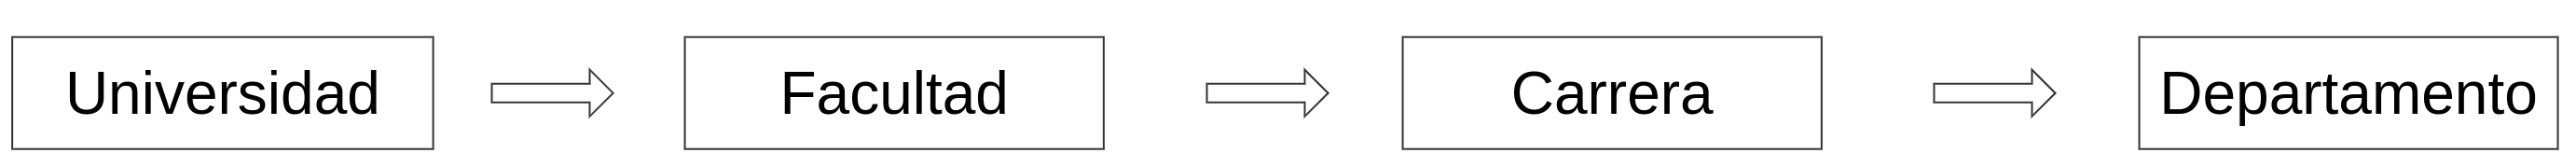
\includegraphics[width=1\linewidth]{images/Chapter 2/department_relation}
	\caption{Relación entre Universidad, Facultad, Carrera y Departamento}
	\label{fig:department_relation}
\end{figure}

\textbf{Asignatura}: Constituye uno de los elementos principales del turno de clases, quién es en definitiva la entidad principal del sistema. Las asignaturas se muestran agrupadas por carreras. Además de cada asignatura se conoce el profesor principal que la imparte.

\textbf{Grupos}: Entidad que se encarga de encapsular conjuntos de estudiantes. Mantiene una relación directa con turno de clase, así como con carrera. 

\textbf{Semestre}: Esta entidad define los diferentes horarios que hay en el sistema. La entidad se llama
“semestre” por convención, pero es configurable la cantidad de semanas de duración, mediante una fecha de inicio y una fecha de culminación. En cada semestre
se pueden estar gestionando un horario diferente. La idea es que cada usuario del sistema tenga acceso al horario del semestre actual, y que el horario del próximo semestre se pueda ir generando simulatáneamente. Cada semestre está compuesto por varias semanas.

\textbf{Semana}: Esta entidad define y se asocia con una semana del año. Cada semana está contenida dentro de un semestre.

\textbf{Tipo de actividad}: Cada uno de los turnos de clase tiene un tipo que resulta importante sobre todo
 para determinar que tipo de aula se necesita. Los tipos más comunes son las conferencias y las clases
 prácticas. Aunque en algunas ocasiones se puede definir además actividades de tipo laboratorio. Es posible generar tipos de actividades nuevas, en caso de que se considere necesario.

\textbf{Profesores}: Es una de las entidades de mayor importancia dentro del sistema. Ofrece una vía para asegurar el manejo de todo lo referente a los profesores del centro. Son considerados usuarios especiales o de más relevancia, pues pueden interactuar directamente con el sistema de horarios, imponiendo restricciones o condiciones sobre el mismo. Todos los profesores están agrupados por departamentos.

\begin{figure}[h!]
	\centering
	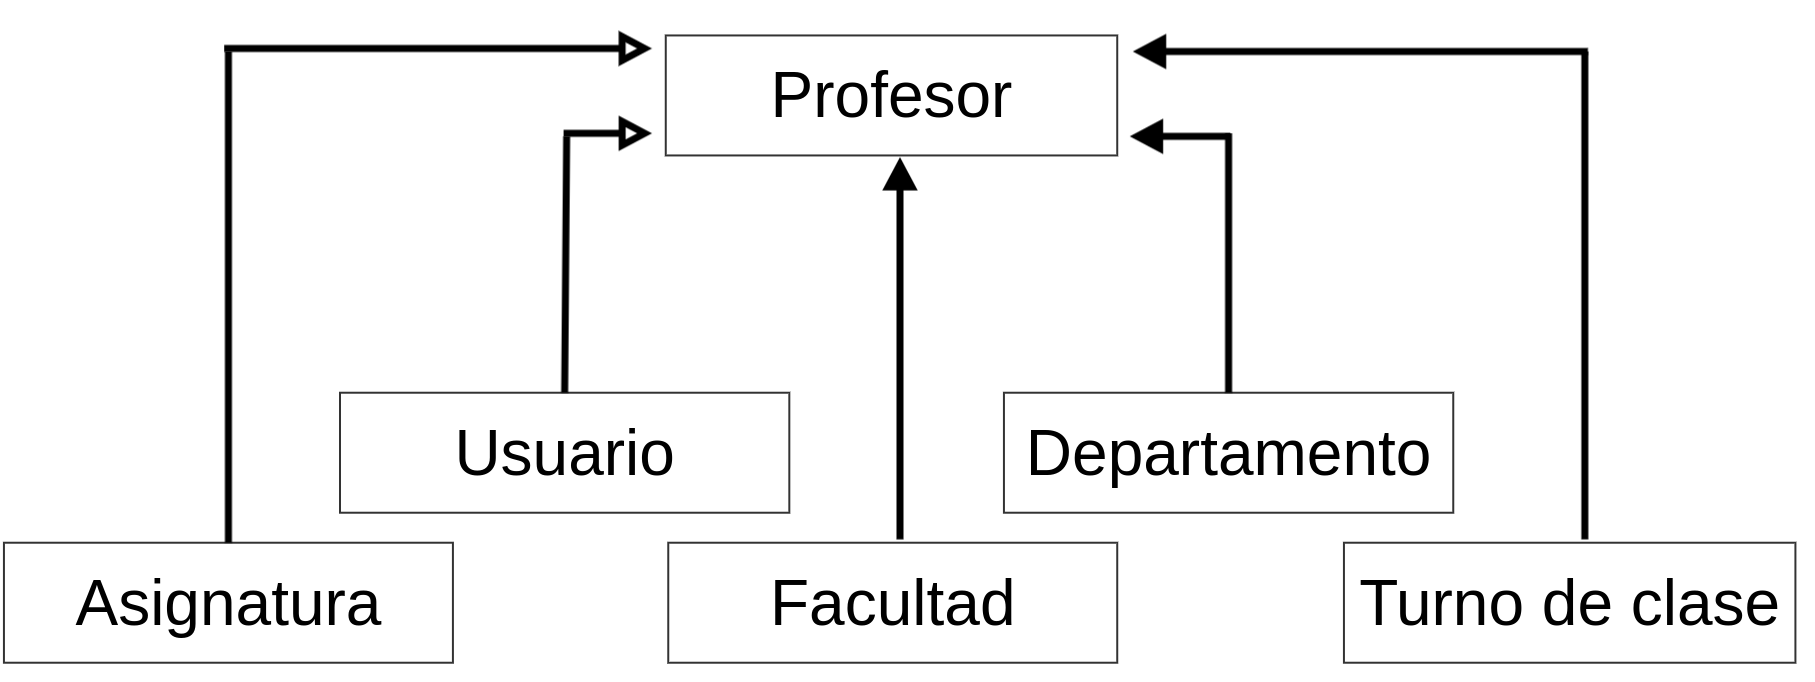
\includegraphics[width=0.75\linewidth]{images/Chapter 2/teacher_relation}
	\caption{Relación de profesor con usuario, asignatura, facultad, turno de clase y departamento }
	\label{fig:teacher_relation}
\end{figure}

\textbf{Local}: Elemento importante que posibilita conocer el lugar donde se impartirá el turno de clase. Es, junto a asignatura y profesor, uno de los elementos principales de un turno de clase. Por lo general a todos los turnos de clases se les
asignará un local. En nuestras universidades existen diferentes tipos de locales: Salones de conferencia,
aulas, laboratorios, anfiteatros, etc. En este sistema los locales se modelaron pertenecientes a una facultad.
Cada uno de los locales se define a partir de un “tipo de local” y esta información es utilizada en algunos de
los algoritmos que se encargan del manejo de las restricciones.

\textbf{Turno de clase}: Es la entidad fundamental del sistema. Maneja todo lo relacionado con las lecciones que se impartirán en cada uno de los días del semestre, por su imporancia se dedicará la sección \ref{sec:classes} al tratamiento de esta entidad en específico.

\textbf{Restricciones}: Entidad que se encarga de manejar las restricciones o condiciones que los profesores y administradores del sistema pudieran imponer sobre el horario. Las restricciones se describen por medio de varios modelos, uno por cada tipo de restricción manejada. Más adelante se dedicará una sección a la descripción detallada de cada uno de los tipos de restricciones manejados.

\textbf{Reportes}: Módulo que posibilita la obtención de un documento en formato \textit{Excel} que puede ser útil para la posterior distribución del horario, o para la revisión del mismo de manera offline. El documento presenta una serie de páginas: una por cada grupo descrito en el horario y una extra que meneja una representación por locales, es decir, la disponibilidad de los mismo durante todo el semestre. En cada página se encuentra descrito el horario por semanas físicas y además se ofrece una leyenda con la descripción de los turnos de clase y la hora de comienzo y finalización de los mismos.\\\\


Cada entidad posee un conjunto de atributos base; por medio de la herencia se logra plasmar esto a la hora de realizar la implementación. 

Todas las entidades del sistema heredan de \texttt{DomainEntity}, que no es más que una \textit{clase abstracta} con un constructor privado y una definición específica de un método \textit{equals}. Esta clase base cuenta además con las propiedades base antes mencionadas. Dichas propiedades son:

\label{props:base}
\begin{itemize}
	\item \textsl{fullName}: Propiedad de tipo texto que almacena el nombre en formato largo del objeto que se esté referenciando en ese momento. 
	\item \textsl{shortName}: Propiedad de tipo texto que almacena el nombre en formato corto del objeto que se esté referenciando en ese momento. 
	\item \textsl{description}: Propiedad de tipo texto que contiene una descripción, que se considere conveniente presentar, acerca del objet que se esté referenciando en ese momento. Esta pripiedad en puede tomar valores nulos.
	\item \textsl{priority}: Propiedad de tipo numérico que almacena la prioridad que pudiera tener un objeto (o entidad) sobre otro en el sistema. Esta propiedad es utilizada principalemte en el cálculo de la \textit{felicidad del sistema}.

\end{itemize}



\section{Modelo entidad-relación (MERX)}


\section{Turno de Clase}
\label{sec:classes}

El \textit{turno de clases} es la entidad fundamental que compone todo sistema de horarios. Como aspecto común a la mayoría de los turnos de clases en universidades cubanas se tiene que estos tienen una duración de 90 minutos y que se pueden clasificar en dos tipos básicos: conferencias y clases prácticas. Cada turno de clases posee una duración por defecto de 90 minutos; este valor es posible cambiarlo para cualquier actividad que se defina dentro del horario. 

En la Universidad de La Habana se estila a separar el día en dos secciones: mañana y tarde y que cada sección esté compuesta por tres turnos de clases, es válido notar que esto se realiza por una especie de convenio ya preestablecido y que el sistema cuenta con las herramientas para variar este funcionamiento. 

Un turno de clases está compuesto por los siguientes atributos:
\begin{itemize}
	\item \textit{Atributos base}: definidos en la sección \ref{props:base}
	\item \textit{Start}: marca la hora de inicio del turno de clase.
	\item \textit{End}: marca la hora de finalización del turno.
	\item \textit{ResourceId}: referente al \texttt{id} del local; se utiliza mayormente en el manejo de la vista asociada a los recursos.
	\item \textit{Week}: referente a la semana de creación del turno de clase.
	\item \textit{Teachers}: colección de elementos que representan los profesores encargados del turno de clases; notar que al menos siempre. se contará con un profesor responsable, que se toma de la asignatura referente al turno.\item \textit{Local}: referente al local donde se impartirá el turno de clase.
	\item \textit{Lesson}: referente a la asignatura.
	\item \textit{TypeClass}: referente al tipo de clase.
	\item \textit{Group}: referente al grupo.
\end{itemize}

Es común notar que en muchos sistemas de horarios, por no decir en todos, contamos con la misma frecuencia de turnos todas las semanas, o a lo sumo en intervalos de quince días. Para ganar en usabilidad y por tanto mejorar la experiencia de usuario se presenta un enfoque que permite crear turnos en una frecuencia específica; dicho en otras palabras y mostrado a través de un ejemplo: si tenemos, dado el caso, que el turno de Matemática Discreta de 2$^{do}$ de Computación se realiza los martes de todas las semanas, en la aplicación no es necesario recorrer todos los martes del semestre e ir creandolos uno por uno, pues se ofrecer una especie de configuración y el sistema se encarga de la posterior creación de cada uno. De cualquier forma también  es posible la creación de turnos individuales sin necesidad de crearlos en serie.

El manejo de turnos en serie nos crea una relación entre los mismos, o sea, los turnos de una misma serie están relacionados entre ellos, esto hace posible que la edición y eliminación de cualquier turno de la serie influya también en el resto de estos turnos. Estas operaciones son además flexibles, dado el hecho de que también es posible modificar inidividualmente los turnos de cualquier serie sin afectar al resto.

El sistema cuenta con una serie de filtros dedicados a obtener secciones del mismo. Los turnos de clase están adaptados, por tanto, a estos requerimientos. Se hace posible agregar filtros por tiempo (día-hora de inicio y finalización), así como por asignaturas, grupos, locales y tipos de clase. 

\section{Manejo de restricciones}

El manejo y gestión de restricciones es un importante \textit{feature} ofrecido en el sistema. Cada profesor propone un conjunto de condiciones que se aplica a los turnos de clase, además de cada profesor se conoce la prioridad, así como la prioridad particular que le otorga a cada restricción. 
Con el objectivo de expresar un concepto un poco más formal: 
\begin{dfn}[Restricción]
	Forma por medio de la cuál los usuarios (principalmente los profesores) expresan sus consideraciones acerca de los elementos que determinan la calidad de cualquier horario propuesto; ya sea en sentido general o personal.
\end{dfn} 

Cada restricción cuenta con un grupo de elementos comunes (figura \ref{fig:base_restrictions}):\\

\paragraph{Condiciones.}
Permite identificar a qué turnos se exigirán determinados requerimientos. Define el filtro inicial que se impone sobre el conjunto de turnos, para obtener así un subconjunto de los mismos, los cuáles deberán cumplir estrictamente los requisitos planteados.\\
	
Una condición está compuesta por un atributo \texttt{A}, y en función de este, un operador \texttt{O} y un valor \texttt{V}. Un atributo relativo a un turno puede ser en realidad, un atributo relativo a una entidad asociada al turno de clase.\\

\begin{table}[h]
	\centering
	\begin{tabular}[c]{l|l|l|r}
		\textbf{Ejemplo}                   & \textbf{Atributo}     & \textbf{Operador} & \textbf{Valor} \\ 
		\hline 
		Aula con más de 30 alumnos         &  Capacidad del Local  & >                 & 30             \\ 
		Ser un martes					   & Día del Turno         & ==                & martes
	\end{tabular}
	\caption{Ejemplos de representación de condiciones}
	\label{tab:conditions}		
\end{table}

Es posible también garantizar el manejo de grupos de condiciones para asegurar que se puedan formular la totalidad de las operaciones deseadas.

\begin{dfn}[Grupo de condiciones]
	Forma amigable de representar un bloque de condiciones lógicas encerradas entre paréntesis; y asegurar, por tanto, la manera correcta de evaluación del mismo. El conjunto de condiciones de una restricción puede verse como un grupo de condiciones.
\end{dfn}

Ejemplos de grupos de condiciones: 
\begin{itemize}
	\item "Ser lunes". Una condición que involucra un solo operador lógico también es considerado un grupo de condiciones.
	\item (Turnos de Matemática Discreta) (del martes). 
	\item (Turnos de Matemática Discreta o del Matemática Numérica) (del martes).
\end{itemize}

\paragraph{Intervalo.}
Ofrece una forma de obtener una separación del  conjunto de turnos en subconjuntos, cada uno conteniendo los turnos correspondientes a un período de tiempo diferente, en cada caso de tamaño \textit{intervalo}, salvo, quizás, el último, en caso de que el curso no pueda ser dividido exactamente en un número 
entero de intervalos de tamaño \textit{intervalo}. El objetivo detrás de esta separación del conjuto de turnos en intervalos, en segregar aún más la evaluación; pues, por ejemplo, supogamos que estamos analizando una restricción sobre $X$ y que: $\exists y \in X $ tal que para $y$ la restricción se incumple, entonces resultaría un poco antiintuitivo decir que la restricción se incumple, solo porque fallara en un turno, por ello si consideramos que $\text{interval} = 7$ (análisis semanal), entonces el turno entraría solo en una semana de las analizadas y por tanto la restricción no se marcaría en su totalidad como incumplida, lo que influiría positivamente en la felicidad del sistema.

\paragraph{Prioridad.}
\label{def:priority}
Establece la prioridad de la restricción. El usuario creador de la restricción (profesor o administrador del sistema) deberá establecer la priridad o cuán importante es la restricción que se está definiendo. Por defecto, si el valor no se proporciona, se fija en 1. Este valor se utilizará posteriormente para el cálculo de la \textit{felicidad} del sistema. La utilidad del mismo radica en gestionar de alguna manera una especie de jerarquía y posibilitar, por tanto un orden, para lograr ser lo más semenjante posible a la vida real.

\paragraph{Descripción.}
Este campo se presenta de manera obligatoria a la hora de la creación de nuevas restricciones. Es un forma de representar con palabras lo que se pretende crear y hacer posible por tanto la rápida comprensión e interpretación de la misma. 

\paragraph{Profesor.}
Se emplea para referenciar al profesor al que está destinada la restricción. En cada de que la restricción sea creada por el profesor en sí, y no por el administrador del sistema, el valor del campo se fijará automáticamente. \\\\

El conjuto de campos definidos por cada tipo de restricción varía en dependencia del tipo.

\begin{figure}[h]
	\centering
	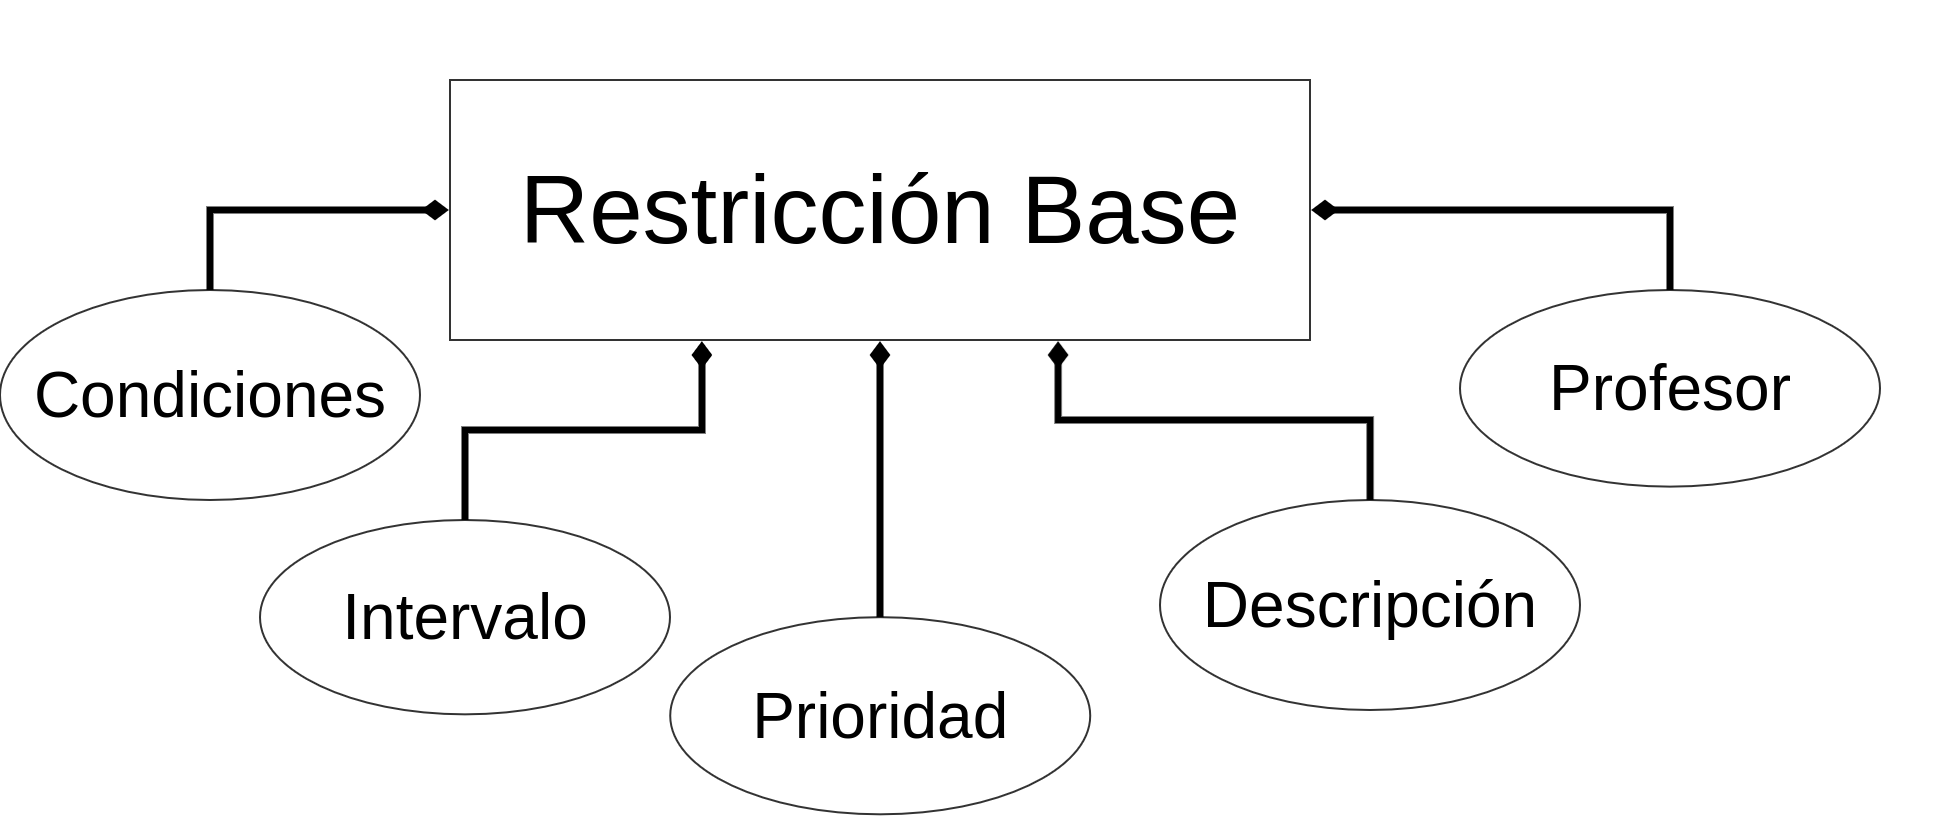
\includegraphics[width=0.75\linewidth]{images/Chapter 2/base_restrictions}
	\caption{Restricción base.}
	\label{fig:base_restrictions}
\end{figure}

\subsection{Tipos de restricciones}

Es posible manejar o declarar diversos timpos de restricciones, dichos tipos ya fueron enunciados en las secciones previas (\ref{state_of_art:restrictions}) de este documento.

\paragraph{Restricción de requerimiento de cuenta simple.}  Esta restricción se refiere al número de turnos que han satisfecho las 
 condiciones fijadas inicialmente. El usuario debe configurar el operador de comparación \textit{O} a aplicar y el valor \textit{V} con el cual comparar. La restricción se cumple si la cantidad de turnos que satisfacen las condiciones mantiene una relación \textit{O} con \textit{V}. El valor de \textit{V} puede ser numérico, porcentual o bien fraccionario  con respecto al total de turnos que pasan la etapa de las condiciones.

\paragraph{Restricción de requerimiento de cuenta de condiciones.} Este requerimiento se refiere a qué parte del conjunto de turnos que ha 
 satisfecho las condiciones previas, cumple también un bloque de condiciones adicionales, y cuenta además con el operador de comparación \textit{O} a aplicar y el valor \textit{V} con el cual comparar. El requerimiento se cumple si la cantidad de turnos que satisfacen las condiciones iniciales y satisfacen simultáneamente otras que se han configurado, mantiene una relación \textit{O} con \textit{V}.

\paragraph{Restricción de requerimiento de distribución de atributos.} Este requerimiento se refiere a la cantidad de valores distintos que puede tomar determinado atributo en el conjunto de turnos que pasa la etapa de condiciones. El usuario configura, además del atributo \textit{A}, el operador de comparación \textit{O} y el valor \textit{V}. El requerimiento se cumple si la cantidad de valores que toma el atributo \textit{A} en el conjunto de turnos que cumple las condiciones previas mantiene una relación \textit{O} con  \textit{V}. En este caso el valor de \textit{V} debe ser numérico.

\paragraph{Restricción de requerimiento relacional.} Este requerimiento se refiere a la relación que mantiene el conjunto de turnos que cumplen las condiciones previas con otro que cumple otro grupo de condiciones. En este caso se requiere que el usuario añada un segundo grupo de condiciones que filtrarán el segundo conjunto de turnos, un atributo \textit{A} y un operador booleano de conjuntos \textit{O} que define la relación entre los valores de \textit{A}
en el primer conjunto y el segundo. El requerimiento se cumple si el conjunto de valores que toma \textit{A} en el primer conjunto de turnos mantiene una relación \textit{O} con el conjunto de valores que toma \textit{A} en el segundo conjunto.

\begin{figure}[h!]
	\centering
	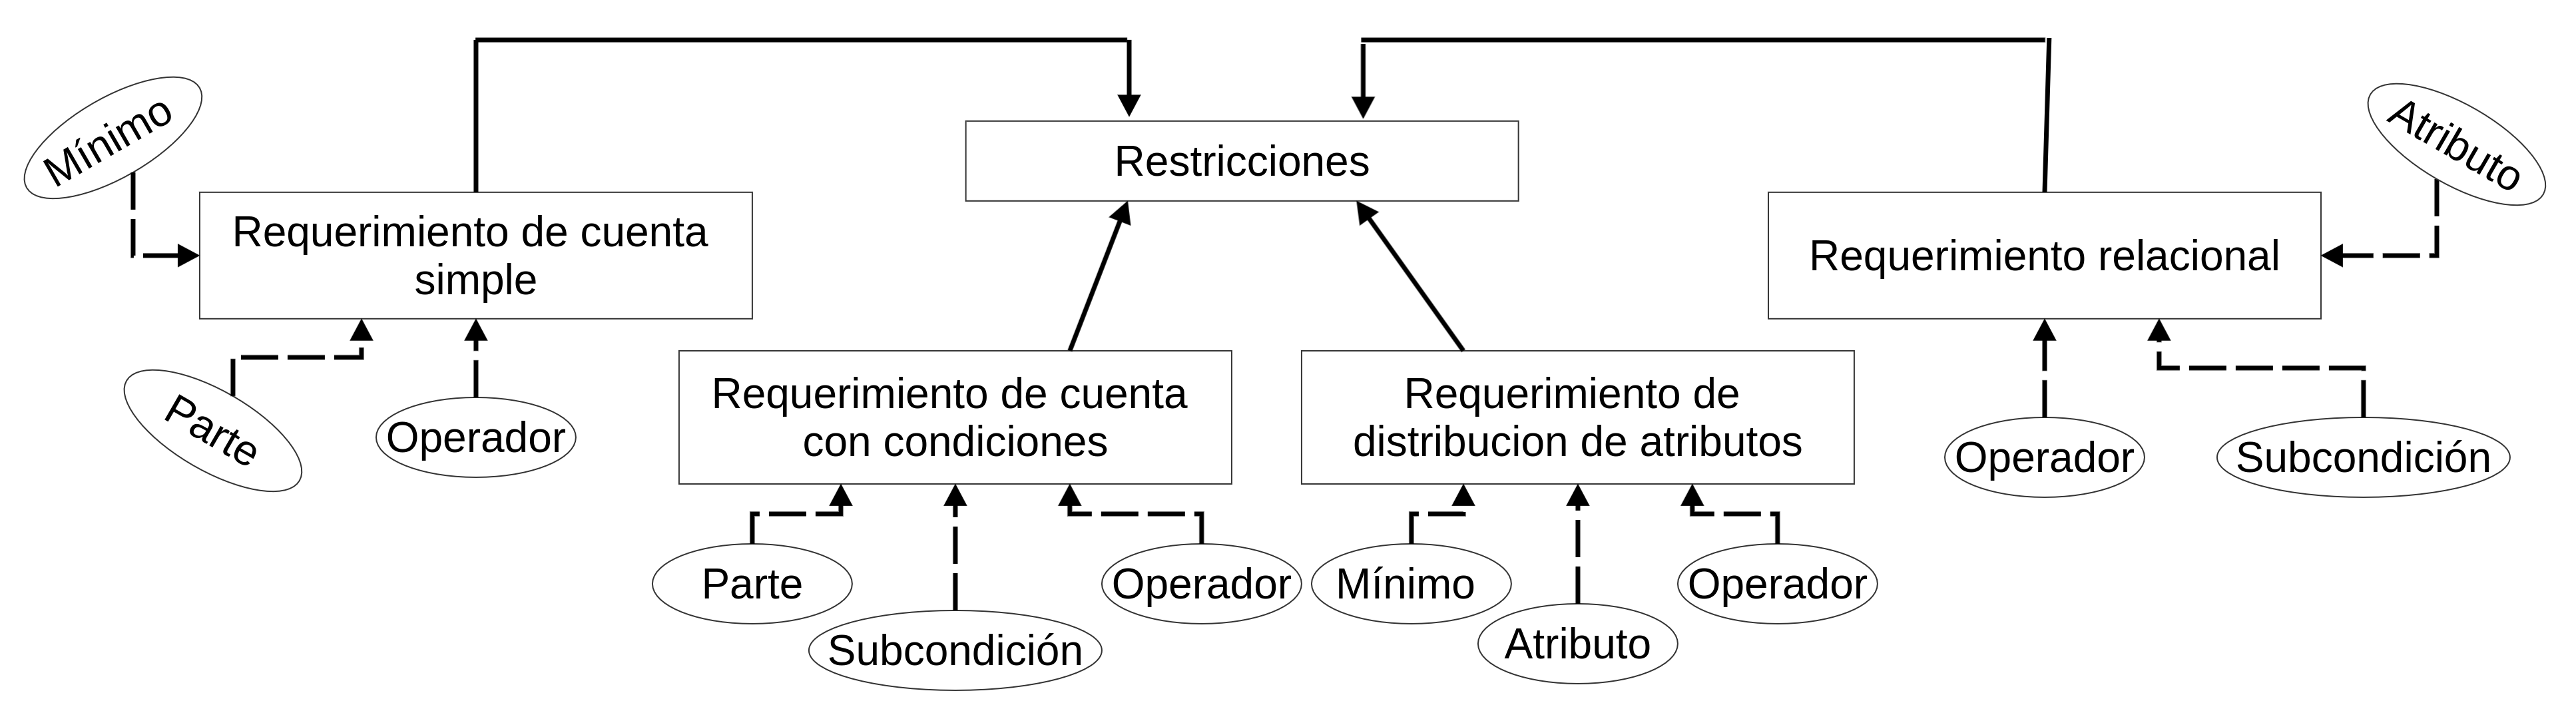
\includegraphics[width=0.95\linewidth]{images/Chapter 2/restrictions}
	\caption{Restricciones con sus atributos.}
	\label{fig:restrictions}
\end{figure}


\subsection{Felicidad del sistema}

La felicidad del sistema, es una cuestión a la que se ha venido haciendo alusión desde los capítulos anteriores. Este valor se obtiene a través de la felicidad relativa a cada uno de los profesores y su posterior procesamiento teniendo en cuenta una fórmula previamente definida.

\begin{dfn} [Felicidad del sistema]
	Valor definido entre 0 y 100 que no es más que un medidor de la calidad del horario.
\end{dfn}

La estrategia utilizada para arribar a las fórmulas de cálculo de felicidad en profesores y en el sistema completo, es básicamente la misma; y se basa en el peso de las prioridades (\ref{def:priority}) establecidas con anterioridad en cada unas de las entidades.

\subsection{Fórmula de la felicidad relativa a un profesor}
Para calcular la felicidad relativa a un profesor con respecto al cumplimiento de sus restricciones, se empleará la siguiente fórmula.

\begin{equation}
	f_p = \frac{w_{1p}c_{1p} + \dots + w_{np}c_{np} }{w_{1p} + \dots + w_{np}}
\end{equation}

\noindent Donde se tiene que: \\

\begin{itemize}
 	\item $w_{ip} \in \mathbb{N}_+ $: Prioridad del requerimiento i-ésimo del profesor p-ésimo
	\item $c_{ip} \in \{0, 1\}$: Cumplimiento del requerimiento i-ésimo del profesor p-ésimo
	\item $n \in \mathbb{N}_+$: Cantidad de requerimientos
	\item $f_p \in [0, 1]$: Felicidad del profesor p-ésimo
\end{itemize}

\subsection{Felicidad relativa al sistema}
Para calcular la felicidad total del sistema se emplea el cómputo de las felicidades respectivas de los profesores:

\begin{equation}
	F_T = \frac{f_1p_1 + \dots + f_mp_m}{p_1 + \dots + p_m}
\end{equation}

\noindent Donde se tiene que:
\begin{itemize}
	\item $f_p \in [0, 1]$: Felicidad del profesor m-ésimo.
	\item $p_m$: Prioridad del profesor m-ésimo.
	\item $m \in \mathbb{N}$: Cantidad de profesores.
\end{itemize}




%Se desarrolló un programa capaz de brindar al usuario la posibilidad de realizar operaciones de inferencia causal. Las características que reúne el programa son las siguientes:
%\begin{enumerate}
%	\item Ofrecer una interfaz visual que permita a usuarios no expertos en programación realizar operaciones de inferencia causal. Dicha interfaz debe asistir al usuario tanto en la creación de los modelos como en las operaciones de inferencia causal, notificándolo en el caso de que existan errores en la entrada provista. 
%	\item Permitir la construcción y visualización de SCMs. Debe permitir además exportar los modelos a ficheros externos para posteriormente ser cargados en el programa.
%	\item Permitir realizar operaciones de inferencia causal sobre modelos causales estructurales. Ofrecer en un menú los distintos tipos de inferencia causal disponibles. Permitir al usuario seleccionar los parámetros que el programa tendrá en cuenta durante la inferencia.
%	\item Ofrecer los resultados correspondientes a la consulta causal especificada por el usuario.
%\end{enumerate}
%
%\section{Implementación}		
%El lenguaje de programación escogido para la implementación fue \textbf{Python} en su versión $3.8$. Su elección se debe a que es un lenguaje de alto nivel, multiparadigma  y con una filosofía que apuesta por un código legible y sencillo.
%
%La implementación de la parte lógica del proyecto consiste de 3 módulos contenidos en un directorio llamado \textit{causality}. Estos módulos son:
%\begin{itemize}
%	\item \textit{main.py}: Contiene la implementación del SCM.
%	\item \textit{tests.py}: Conjunto de tests unitarios destinados a probar las componentes fundamentales de la implementación.
%	\item \text{util.py}: Conjunto de métodos auxiliares que serán utilizados desde otros módulos.
%\end{itemize}
%
%\subsection{Implementación del modelo causal estructural}
%En el módulo \textit{main.py} se trabaja con un conjunto de clases para la implementación del modelo:	  
%
%\begin{lstlisting}
%	class Variable:
%		def __init__(self, name, values):...
%	
%	class ExogenousVariable(Variable):
%		def __init__(self, name, values, distribution):...
%	
%	class EndogenousVariable(Variable):
%		def __init__(self, name, values, parents, expression):...
%	
%	class SCM:
%		def __init__(self, exogenous_variables, endogenous_variables):...
%\end{lstlisting}
%
%La clase \textit{Variable} reúne las características comunes de las variables tanto exógenas como endógenas. Debe proveerse un nombre para la variable que la identifique en el modelo, por lo que este debe ser único. Además debe proveerse una lista de los valores que la variable puede tomar. La naturaleza de las variables es discreta y estas solo pueden tomar valores numéricos. Esta clase no se utiliza directamente sino que es heredada por las clases \textit{ExognousVariable} y \textit{EndogenousVariable}. 
%
%La clase \textit{ExogenousVariable} representa a las variables exógenas de un SCM. Para crear una variable exógena se debe especificar su nombre, los valores que toma y su distribución de probabilidad. Dicha distribución consiste en una lista $P$ donde cada valor $P[i]$ se corresponde con la probabilidad de que la variable tome el valor $V[i]$, donde $V$ es la lista de valores provista. La lista debe cumplir con todas las propiedades de una distribución de probabilidad:
%\begin{itemize}
%	\item La suma de sus valores debe ser igual a 1
%	\item Cada valor debe ser encontrarse en el intervalo $[0,1]$
%\end{itemize}
%
%En el caso de las variables endógenas, representadas por la clase \textit{EndogenousVariable} debe especificarse el nombre, los valores que toma, los padres de la variable (variables de las que depende) y la expresión que define a la misma. Es importante especificar todos los posibles valores que puede tomar la variable a partir de las variables de las que depende. Toda variable endógena debe depender de al menos otra variable y una de estas variables debe ser exógena. Esto último es necesario para el cálculo correcto de los contrafactuales, ya que el método utilizado (redes gemelas) utiliza las variables exógenas para conectar las variables del mundo real con las del mundo alternativo.
%
%La expresión que define a la variable será una cadena con una sintaxis similar a las expresiones de Python. Además se podrán usar funciones de la clase \textit{math}, que viene integrada a dicho lenguaje. Ejemplo de posibles expresiones válidas son:
%\begin{itemize}
%	\item X + Y - 1
%	\item (X and Y) if Z == 0 else (X or Y)
%	\item max(X, Y) - min(X,Y)
%\end{itemize}
%Las variables que aparecen en las expresiones deben corresponderse con los nombres de las variables de las que depende la variable que se está definiendo.
%
%Una vez creadas las variables exógenas y endógenas, estas se agrupan en dos listas y se llama al constructor de la clase $SCM$, la cual representa a los modelos causales estructurales.
%
%Por ejemplo, si se tiene un modelo como el siguiente:
%
%\begin{model}
%	\label{model:sum}
%	\[
%	\arraycolsep=10pt
%	\begin{array}{ccc}
%		U = \{Ux, Uy, Uz\}&
%		V = \{X, Y, Z\}&
%		E = \{f_x, f_y, f_z\}
%	\end{array}
%	\]
%	
%	\[Val(Ux)=Val(Uy)=Val(X)=Val(Y)=\{0,1,2\}\]
%	\[Val(Uz)=\{0, 1\}\]
%	\[Val(Z)=\{0, 1, 2, 3, 4\}\]
%	
%	\begin{equation*}
%		P(X=x)=  
%		\left\{
%		\begin{array}{ll}
%			0.1 & \mathrm{si\ } x = 0\\
%			0.2 & \mathrm{si\ } x = 1\\
%			0.7 & \mathrm{si\ } x = 2\\
%		\end{array}
%		\right\}.
%	\end{equation*}
%	
%	\begin{equation*}
%		P(Y=y)=  
%		\left\{
%		\begin{array}{ll}
%			0.2 & \mathrm{si\ } y = 0\\
%			0.2 & \mathrm{si\ } y = 1\\
%			0.6 & \mathrm{si\ } y = 2\\
%		\end{array}
%		\right\}.
%	\end{equation*}
%	
%	\begin{equation*}
%		P(Z=z)=  
%		\left\{
%		\begin{array}{ll}
%			0.8 & \mathrm{si\ } z = 0\\
%			0.2 & \mathrm{si\ } z = 1\\
%		\end{array}
%		\right\}.
%	\end{equation*}
%	
%	\begin{center}
%		\[
%		\begin{array}{cc}
%			f_x: & X = Ux\\
%			f_y: & Y = Uy\\	
%		\end{array}
%		\]			
%		\begin{equation*}
%			f_z: Z=  
%			\left\{
%			\begin{array}{ll}
%				X + Y & \mathrm{si\ } Uz = 0\\
%				X * Y & \mathrm{si\ } Uz = 1\\
%			\end{array}
%			\right\}.
%		\end{equation*}
%	\end{center}
%\end{model}
%
%Entonces para construir dicho modelo se usaría el código:
%
%\begin{lstlisting}
%	Ux = ExogenousVariable("Ux", [0, 1, 2], [0.1, 0.2, 0.7])
%	Uy = ExogenousVariable("Uy", [0, 1, 2], [0.2, 0.2, 0.6])
%	Uz = ExogenousVariable("Uz", [0, 1], [0.8, 0.2])
%	
%	X = EndogenousVariable("X", [0, 1, 2], [Ux], "X")
%	Y = EndogenousVariable("Y", [0, 1, 2], [Uy], "Y")
%	Z = EndogenousVariable("Z", [0, 1, 2, 3, 4], [X, Y, Uz], "X + Y if Uz == 0 else X * Y")
%	
%	model = SCM([Ux, Uy, Uz], [X, Y, Z])
%\end{lstlisting}
%
%Los modelos también tienen una representación en formato JSON (Javascript Object Notation) con el objetivo de persisitirlos en ficheros y así poder usarlos posteriormente. El método \textit{export\_to\_json} convierte un objeto de tipo SCM a su representación en JSON, mientras que el método \textit{import\_from\_json} crea un objeto de tipo SCM a partir de la representación en JSON correspondiente. A su vez, los métodos \textit{export\_to\_json\_file} e \textit{import\_from\_json\_file} permiten guardar y cargar de memoria externa respectivamente.
%
%\subsection{Algoritmos de inferencia}
%La implementación de los algoritmos de inferencia causal se basa en la inferencia bayesiana. A la hora de responder a una pregunta causal se aplica un algoritmo que en algún punto pasa por la construcción de una red bayesiana y la ejecución de un algoritmo de inferencia para obtener la respuesta deseada.
%
%Para el trabajo con redes bayesianas se utilizó la librería \textbf{pgmpy} \cite{ankan2015pgmpy}. Esta es una librería de código abierto para el trabajo con redes bayesianas, enfocada en la modularidad y la extensibilidad. Contiene implementaciones de algoritmos de estimación de parámetros, aprendizaje de estructura, inferencia exacta, aproximada y además inferencia causal.
%
%El método \textit{build\_bayesian\_network} construye una red bayesiana a partir de un modelo causal estructural, mediante un proceso similar al descrito en la sección \ref{secc:scm-bn}. La parte más compleja de dicho algoritmo consiste en la creación de las tablas de probabilidad de las variables endógenas, donde es necesario computar todas las combinaciones posibles de valores que pueden tomar los padres más la variable. Así, si una variable $X$ depende de un conjunto $Pa_X=\{P_1, P_2, ..., P_n\}$ de variables, su tabla de probabilidad contaría con $|X| \cdot \prod_{i=1}^n |P_i|$ entradas, donde $|P_i|$ denota la cardinalidad de la variable $P_i$ y $|X|$ la cardinalidad de $X$. Para determinar el valor de cada probabilidad $P(X_i=x_i \mid Pa_X=x^{\ast})$ se evalúa la expresión que define a $X$ en la correspondiente asignación $x^{\ast}$ a las variables padres de $X$. Si el resultado es igual a $x_i$, entonces la probabilidad toma valor 1. En caso contrario toma valor 0. Para evaluar la expresión se utiliza la función \textit{eval} integrada a Python, que toma una expresión en forma de cadena de caracteres y los valores que se le asigna a las variables, y devuelve el resultado de evaluar dicha expresión.
%
%Existen 3 tipos principales de inferencia en la implementación: predicciones, intervenciones y contrafactuales. Las signaturas de los métodos correspondientes a dichas operaciones se definen a continuación:
%
%\begin{lstlisting}
%	def predict(self, variables, observations={}, map=False, joint=False, algorithm="BP"):...
%	
%	def do_bayesian(self, variables, do_variables, observations={}, map=False, joint=False, algorithm="BP"):...
%	
%	def counterfactual(self, variables, do_variables, observations={}, map=False, joint=False, algorithm="BP"):...
%\end{lstlisting}
%
%El método \textit{predict} permite realizar una predicción en el modelo, devolviendo las probabilidades actualizadas de un conjunto de variables solicitadas (parámetro \textit{variables}) a partir de un conjunto de variables observadas (\textit{observations}). Por ejemplo, si se quiere determinar la probabilidad $P(Y \mid X=1)$ se hece la llamada siguiente al método:	
%\begin{lstlisting}
%	result = model.predict(["Y"], observations={"X": 1})
%\end{lstlisting}	
%El método \textit{do\_bayesian} calcula el resultado de una intervención, incorporando el parámetro \textit{do\_variables} que indica las variables que son intervenidas y los valores que son forzados a tomar. Suponiendo que se quiere calcular $P(Y \mid do(X=1), Z=2)$ la llamada al método sería:
%\begin{lstlisting}
%	result = model.do_bayesian(["Y"], {"X": 1}, observations={"Z": 2})
%\end{lstlisting}
%
%Para calcular el resultado de la intervención se usa el procedimiento descrito en la sección \ref{sec:do-bn}: se construye el submodelo correspondiente a la intervención mediante el método \textit{get\_submodel}, y convirtiéndolo en red bayesiana con el método \textit{build\_bayesian\_network} se aplica inferencia para obtener la respuesta deseada. 
%
%El método \textit{counterfactual} calcula el resultado de un contrafactual, recibiendo los mismos parámetros que el método \textit{do\_bayesian} pero con un significado ligeramente distinto: las variables de la respuesta deben corresponder al mundo alternativo, para lo cual se debe añadir el caracter \textquoteleft*\textquoteright al final del nombre de la variable, y lo mismo ocurre con las variables especificadas en \textit{do\_variables} que corresponden a las intervenciones realizadas en el mundo alternativo. Para calcular el contrafactual $P(Y_{X=1} \mid Z=z)$ la llamada al método \textit{counterfactual} sería:
%\begin{lstlisting}
%	result = model.counterfactual(["Y*"], {"X*": 1},observations={"Z": 2})
%\end{lstlisting}
%Para calcular el contrafactual se utiliza el método de las redes gemelas descrito en la sección \ref{sec:tn}. Se construye la estructura mediante el método \textit{build\_twin\_network} que a partir de un modelo construye el modelo de redes gemelas correspondiente. La respuesta al contrafactual se obtiene llamando al método \textit{do\_bayesian} sobre el modelo de redes gemelas resultante.
%
%Los métodos anteriores disponen de un conjunto de parámetros opcionales . El parámetro \textit{map} especifica si en vez de realizar inferencia probabiliística se debe realizar inferencia MAP. El parámetro \textit{joint} indica si se desea obtener en la respuesta la distribución de probabilidad conjunta o las distribuciones por separado. El parámetro \textit{algorithm} indica el algoritmo de inferencia que será usado y puede tomar dos valores: \textquotedblleft BP \textquotedblright(propagación de creencias) y \textquotedblleft VE\textquotedblright(eliminación de variables).	
%
%En caso de que la inferencia especificada sea probabilística, los métodos \textit{predict}, \textit{do\_bayesian} y \textit{counterfactual} devuelven una función. Si es solicitada la distribución conjunta, esta recibe como parámetro una asignación en forma de diccionario de los valores que toma cada variable y devuelve la probabilidad correspondiente. Si no se pide la distribución conjunta, entonces la función devuelta recibe como parámetro el nombre de una variable de la respuesta y el valor que toma, devolviendo la probabilidad correspondiente. Por otro lado, si se especifica que la inferencia es de tipo MAP, entonces se devuelve un diccionario con la asignación más probable a las variables.
%
%Por ejemplo, para el modelo \ref{model:sum}, si deseamos obtener el valor de $P(Z_{X=1}=3 | Z=3)$, la instrucción de código quedaría:
%\begin{lstlisting}
%	model.counterfactual(["Z*"], {"X*": 1}, {"Z": 3})("Z*", 3)
%\end{lstlisting}
%En cambio la probabilidad conjunta $P(Z=3, Y=2 | do(X=1))$ se obtendría así:
%\begin{lstlisting}
%	model.do_bayesian(["Z", "Y"], {"X": 1})({"Z": 3, "Y": 2})
%\end{lstlisting}
%Por otro lado la asignación más probable MAP($Z, Y | do(X=1)$) se obtendría leyendo el diccionario que devuelve el llamado al método \textit{do\_bayesian\_map}:
%\begin{lstlisting}
%	result = model.do_bayesian(["Y", "Z"], {"X": 1}, map=True)
%	for variable, value in result.items():
%		print(variable, value)
%\end{lstlisting}
%
%Como se vio en las secciones \ref{sec:attr} y \ref{sec:med}, las fórmulas de mediación y atribución se definen en términos de intervenciones y contrafactuales y por tanto su implementación es inmediata. En el caso de la atribución se reciben dos parámetros correspondientes al tratamiento(causa) y la respuesta(efecto). Cada uno de estos parámetros consiste en una tupla de tres elementos de la forma (nombre de la variable, valor verdadero, valor falso):
%
%\begin{lstlisting}
%	def prob_of_neccesity(self, cause, effect):...
%	
%	def prob_of_sufficiency(self, cause, effect):...
%	
%	def prob_of_neccesity_and_sufficiency(self, cause, effect):...
%\end{lstlisting}
%
%Por ejemplo si se tienen dos variables binarias $X$, $Y$, y se quiere calcular la necesidad de tomar un medicamento($X=1$) para recuperarse ($Y=1$), entonces el llamado al método \textit{prob\_of\_neccesity} sería:
%
%\begin{lstlisting}
%	model.prob_of_neccesity(self, ("X", 1, 0), ("Y", 1, 0))
%\end{lstlisting}
%
%Las fórmulas de mediación implementadas son el efecto total y el efecto directo controlado, que aplican para dos pares de variables cualesquiera:
%
%\begin{lstlisting}
%	def total_effect(self, cause, effect_variable):...
%	
%	def controlled_direct_effect(self, cause, effect_variable, mediator):...
%\end{lstlisting}
%
%Ambas reciben un parámetro \textit{cause} que consiste en una tupla (nombre de la causa, valor inicial, valor final) y otro parámetro \textit{effect\_variable} que indica el nombre de la variable en la que se mide el efecto. Si quisiésemos medir el efecto total de $X$ en $Y$ cuando $X$ cambia de $0$ a $1$, entonces llamaríamos a la primera función con los parámteros:
%\begin{lstlisting}
%	model.total_effect(("X", 0, 1), "Y")
%\end{lstlisting}
%
%El efecto directo controlado recibe otro parámetro que consiste en una tupla (nombre, valor) correspondiente al mediador que se está analizando. Una posible llamada al método sería:
%\begin{lstlisting}
%	model.controlled_direct_effect(("X", 0, 1), "Y", ("Z", 0))
%\end{lstlisting}
%Aquí se calcula el efecto de $X$ en $Y$ cuando el mediador $Z$ es obligado a tomar el valor $0$.
%
%\subsection{Complejidad}
%La complejidad de los algoritmos de inferencia causal es exponencial ya que todos utilizan un algoritmo de inferencia bayesiana exacta que puede ser propagación de creencias \cite{lauritzen1988local}, cuya complejidad es exponencial con respecto al tamaño del mayor clique del grafo moral triangulado, o eliminación de variables \cite{zhang1994simple}, cuya solución pasa por encontrar un conjunto de variables de eliminación óptimo, siendo este un problema NP-completo.
%
%\begin{dfn}
%	Sea $G = \langle V, E \rangle$ un grafo dirigido donde $N = |V|$ y $M = |E|$. El coeficiente de densidad de $G$ es:
%	\[D_G = \frac{M}{N^2}\]
%\end{dfn}
%
%\begin{dfn}
%	Un grafo $G$ es esparcido si $D_G \le 0.08$. En caso contrario se dice que es denso.
%\end{dfn}
%
%El tiempo de ejecución de los algoritmos depende de varios factores: el número de nodos o tamaño del grafo, la densidad del grafo y la cantidad máxima de valores que puede tomar cada variable. Se obtuvieron resultados satisfactorios para grafos esparcidos y con variables que toman un número pequeño de valores.
%
%Los tiempos de ejecución obtenidos para las predicciones fueron muy similares a los de las intervenciones. Esto tiene sentido, puesto que una predicción es una intervención sobre un conjunto vacío de variables. 
%
%En las predicciones se comportó ligeramente mejor el algoritmo de propagación de creencias que el de eliminación de variables. La Figura \ref{fig:p-24} compara el comportamiento de los dos, tiendo en cuenta distintas cardinalidades máximas para las variables del modelo (valor de $v$).  La Figura \ref{fig:p-bp-8-60} muestra el comportamiento de las predicciones usando el algoritmo de propagación de creencias en modelos de hasta 60 variables donde todas son binarias.
%
%\begin{figure}[h!]
%	\centering
%	\begin{subfigure}{.49\linewidth}
%		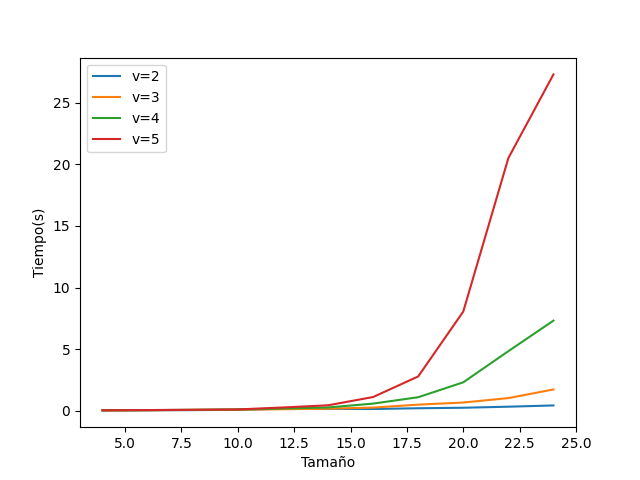
\includegraphics[width=\linewidth]{./images/Chapter-3/p-bp-8-24}
%		\caption{BP}
%	\end{subfigure}
%	\begin{subfigure}{.49\linewidth}
%		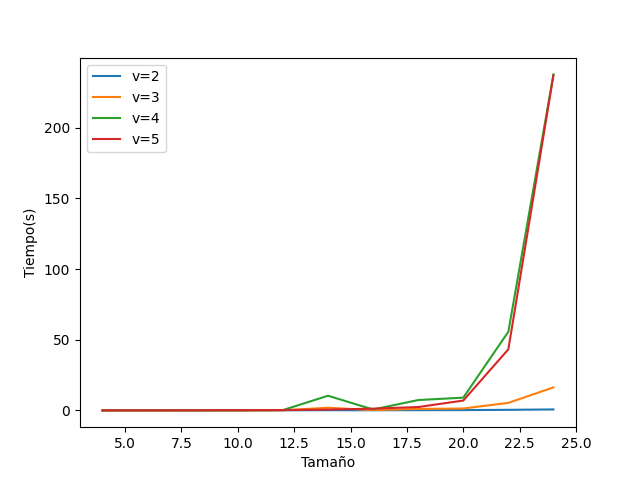
\includegraphics[width=\linewidth]{./images/Chapter-3/p-ve-8-24}
%		\caption{VE}
%	\end{subfigure}
%	\caption{Comparación entre los algoritmos de propagación de creencias y eliminación de variables}
%	\label{fig:p-24}
%\end{figure}
%
%\begin{figure}[h!]
%	\centering
%	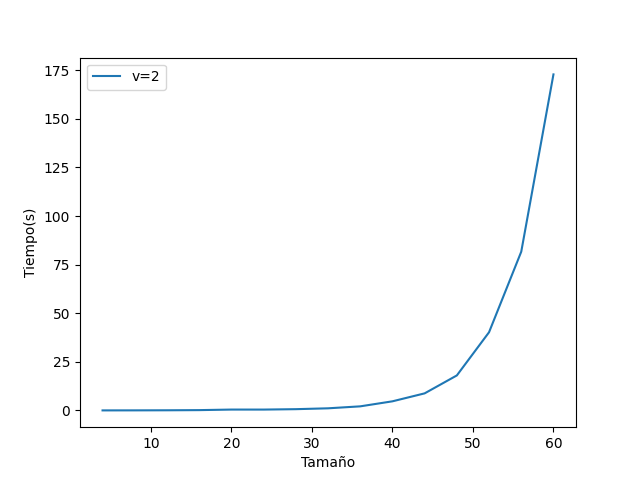
\includegraphics[width=0.5\linewidth]{./images/Chapter-3/p-bp-8-60}
%	\caption{Comportamiento del algoritmo de propagación de creencias para modelos con sólo variables binarias}
%	\label{fig:p-bp-8-60}
%\end{figure}
%
%Los contrafactuales resultaron ser viables en redes más pequeñas que las de las predicciones e intervenciones, pues el método de las redes gemelas transforma la red en una de casi el doble de su tamaño y realiza inferencia sobre ella. En la Figura \ref{fig:c-8-20} se muestra el comportamiento de los contrafactuales en dependencia del algoritmo que se use durante la fase de inferencia bayesiana en modelos con solo variables binarias.
%
%\begin{figure}[h!]
%	\centering
%	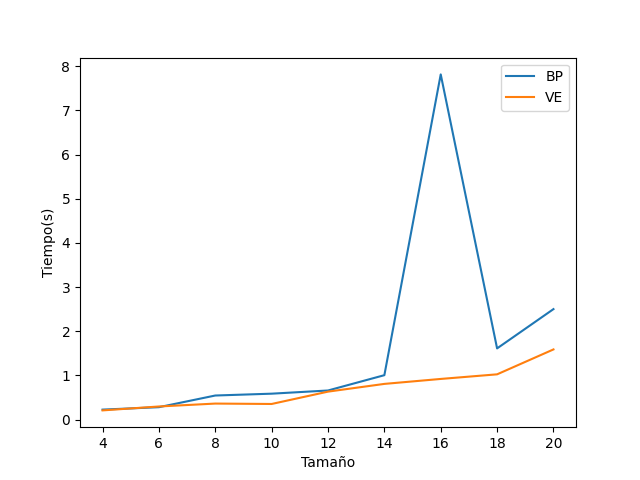
\includegraphics[width=0.5\linewidth]{./images/Chapter-3/c-8-20}
%	\caption{propagación de creencias vs eliminación de variables en contrafactuales}
%	\label{fig:c-8-20}
%\end{figure}
%
%
%
%
%\section{Interfaz de usuario}
%La interfaz de usuario está concebida para facilitar el uso de la inferencia causal en problemas que lo requieran, abstrayendo al usuario del ambiente de la programación. Se brinda al usuario la posibilidad de crear, editar, cargar y guardar modelos estructurales causales. Además es posible visualizar el grafo causal asociado. Se brindan 5 modalidades de inferencia causal: predicción, intervención, contrafactual, atribución y mediación. Para cada tipo de inferencia se provee un formulario donde el usuario especifica los parámetros de la consulta a realizar. Para asegurar que la entrada provista por los usuarios al programa es la correcta, en todos los formularios existen métodos de validación que notifican al usuario en caso de que la entrada sea incorrecta.
%
%La interfaz visual fue desarrollada con la librería \textbf{kivy}\cite{kivyDocs}. Entre sus principales características se encuentran que es de código abierto, multiplataforma y eficiente. Permite la creación de aplicaciones de manera rápida y a diferencia de otras librerías para interfaces visuales como PyQt, ofrece una sintaxis más elegante, al estilo de Python.
%
%Para la visualización de los grafos causales se utilizaron dos librerías: \textbf{pydot}\cite{pydotDocs} y \textbf{networkx}\cite{networkxDocs}. Ello se debe a que en algunas arquitecturas de sistemas operativos la primera, que es la preferida, requiere de la instalación de dependencias adicionales, y no se desea que esa tarea recaiga en manos del usuario. Por ello cuando se solicita la imagen de un grafo causal, se da prioridad a \textit{pydot}, y en caso de que no sea posible utilizarla, se usa la segunda, que es más flexible.
%
%Por último, para el proceso de empaquetado del software se utilizó \textbf{PyInstaller}\cite{PyInstaller}. Esta librería agrupa el código y las dependencias en un paquete que puede ser usado en otras computadoras sin la necesidad de instalar un intérprete de Python ni las dependencias, siempre y cuando sea en un sistema operativo similar a donde se construyo el paquete.
%
%\begin{figure}
%	\centering
%	\begin{subfigure}{\linewidth}
%		\centering
%		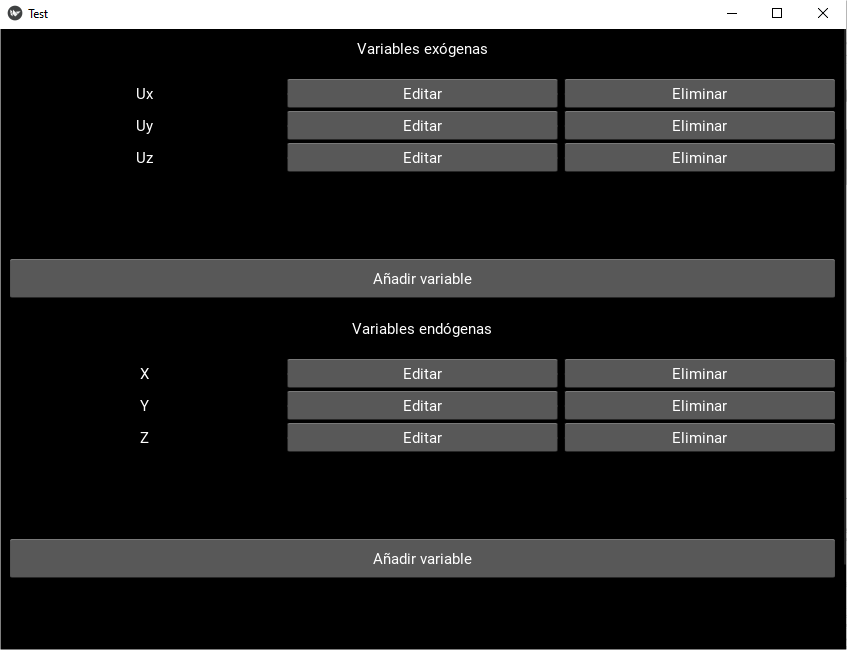
\includegraphics[width=300px, height=280px]{./images/Chapter-3/create-model}
%		\caption{Ventana de creación de un modelo causal estructural}
%		\label{fig:create-model}
%	\end{subfigure}
%	\begin{subfigure}{\linewidth}
%		\centering
%		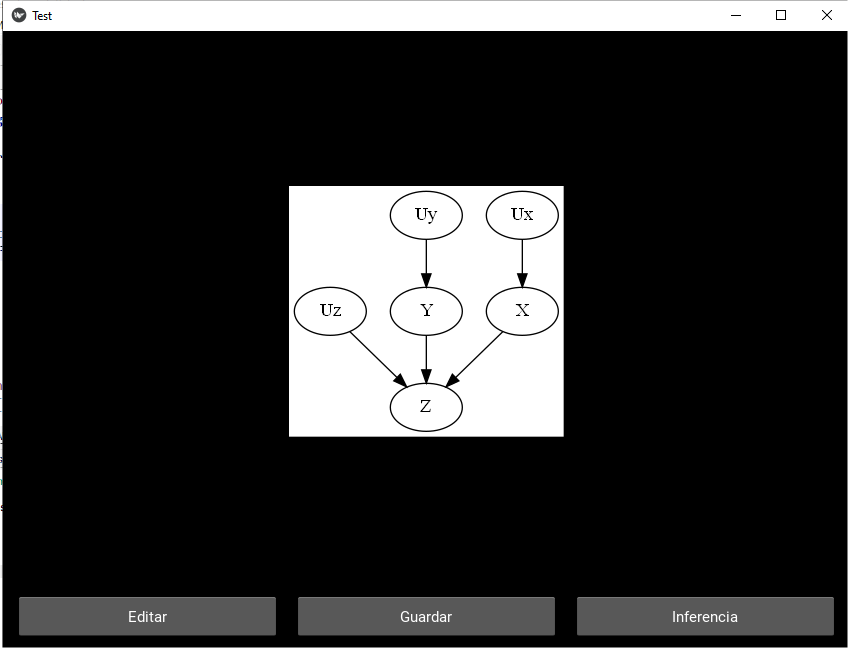
\includegraphics[width=300px, height=280px]{./images/Chapter-3/model-view}
%		\caption{Ventana principal del modelo}
%		\label{fig:model-view}
%	\end{subfigure}
%\end{figure}
%
%\begin{figure}
%	\begin{subfigure}{\linewidth}
%		\centering
%		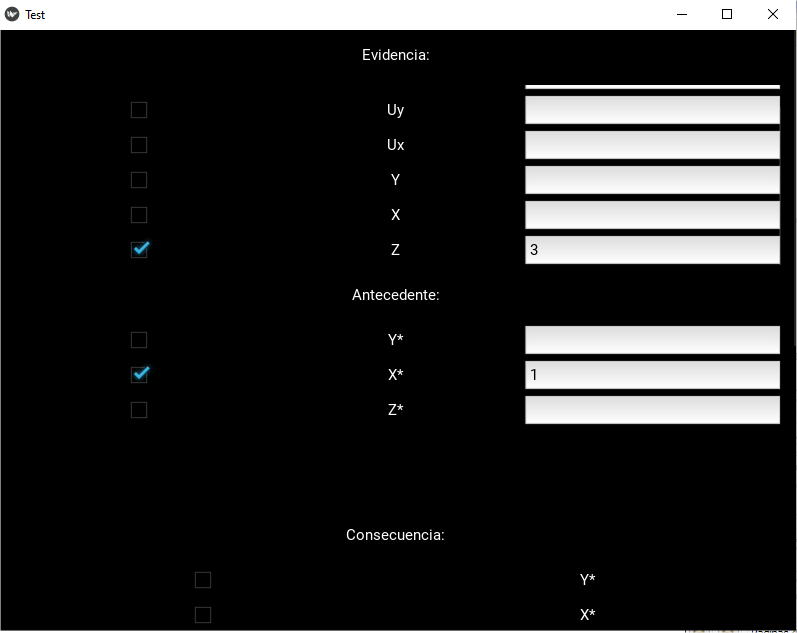
\includegraphics[width=300px, height=280px]{./images/Chapter-3/counterfactual(1)}
%		\subcaption{}
%		\label{fig:counterfactual-1}
%	\end{subfigure}
%	\begin{subfigure}{\linewidth}
%		\centering
%		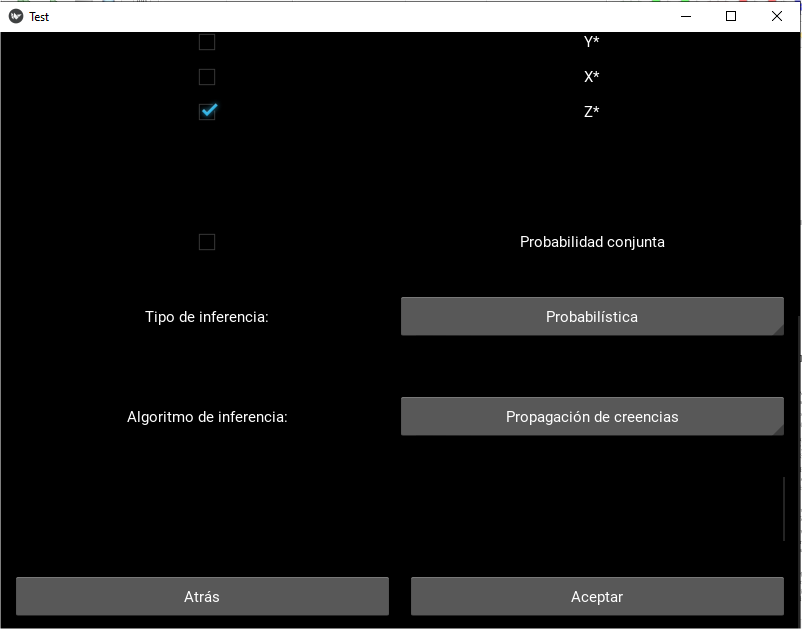
\includegraphics[width=300px, height=280px]{./images/Chapter-3/counterfactual(2)}
%		\subcaption{}
%		\label{fig:counterfactual-2}
%	\end{subfigure}
%	\subcaption{Formulario para calcular un contrafactual}
%	\label{fig:counterfactual}
%\end{figure}
%
%\begin{figure}
%	\centering
%	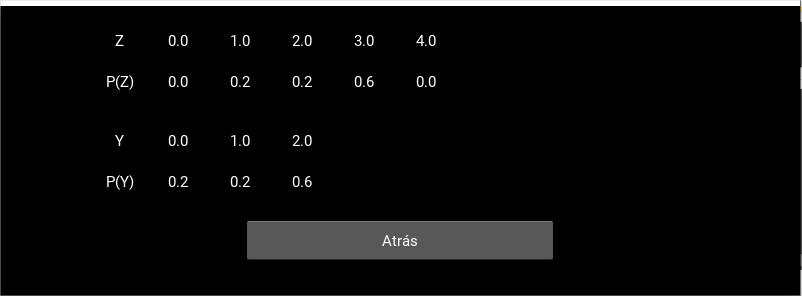
\includegraphics[width=300px, height=280px]{./images/Chapter-3/intervention-result}
%	\caption{Resultados de una intervención}
%	\label{fig:intervention}
%\end{figure}